\section{Análisis de Clusters}

\noindent Según \emph{Jain,A.K. y Richard, C.D; }\cite{Jain 1988} el análisis de cluster es un conjunto de técnicas exploratorias las cuales toman un conjunto de datos provenientes de hacer observaciones simultaneas  sobre un vector aleatorio $\mathbf{x}$ de tamaño $p$. Estas técnicas lo que buscan es realizar agrupaciones de los datos. Lo bueno de estos métodos es que no requieren las suposiciones habituales de otros métodos.

\noindent Para empezar, debemos definir que es un \emph{cluster}
\begin{defi}
Diremos que un cluster o conglomerado es un subconjunto de las observaciones que son similares entre sí \cite{Everitt 2011}. Esta definición la damos ya que nos centraremos en agrupar observaciones y no variables. 
\end{defi}

\noindent Es fácil observar que los clusters definen la siguiente relación de equivalencia $\mathcal{R}$ en la que dos observaciones, $\mathbf{x}_i,\mathbf{x}_{i'}, i,i'=1 \ldots N$ están relacionadas si pertenecen al mismo clúster \cite{Cuadras 2014}. Por tanto, cada cluster genera una clase de equivalencia $[c_c], c=1\ldots C$ donde $C$ es el número de clusters

\noindent El conjunto de clusters generan un clustering o partición es decir
\begin{defi}
Se llama \textit{clustering} a la partición que provoca la relación $\mathcal{R}$ del espacio de observaciones. 
\end{defi}

\noindent Para llegar a dichas particiones podemos usar distintos tipos de algoritmos según el número de particiones que se generen a lo largo del proceso \cite{Jain 1988}
\begin{itemize}
\item \emph{Particional}, si el proceso únicamente genera una partición del espacio 
\item \emph{Jerárquico}, si el proceso genera una secuencia anidada de particiones que dependiendo de cómo se desarrolle puede ser de los siguientes tipos:
\begin{itemize}
\item \emph{Aglomerativo} si empieza con una partición con tantos clusters como y en cada paso se unen los que cumplan algún criterio 
\item \emph{Divisivo} si se empieza con un único cluster el cual se van separando según alguna condición
\end{itemize}
\end{itemize}

\noindent En resumen, el análisis de cluster es un conjunto de técnicas que permiten la simplificación estructural de las observaciones recogidas de un vector aleatorio mediante la agrupación de las mismas en conjuntos llamados clusters \cite{Everitt 2011}. 

\noindent El análisis de clusters ha sido aplicado en infinidad de áreas como el marketing con el objetivo de segmentar los anuncios \cite{Okazaki 2006}, la psicología para detectar si se da un sólo trastorno en una población \cite{Everitt 2002} o en el caso de la medicina para intentar estudiar la supervivencia de pacientes con carcinoma renal \cite{Witten 2010}. Estos son ejemplos de unos pocas aplicaciones, pero también nos pueden ayudar en la predicción del riesgo crediticio, segmentación electoral etc... 
\subsection{Algoritmos Jerárquicos}

\noindent Los algoritmos jerárquicos son aquellos que utilizan como entrada no la matriz de los datos per sé, en su lugar, estas utilizan como entrada la matriz de distancias o similaridad.

\noindent Un algoritmo jerárquico genera una secuencia de particiones o clustering de la siguiente manera 
\begin{defi}
Una partición del espacio $\Pi^{(r)}$ está anidada en otra partición $\Pi^{(k)}$ y se denota $\Pi^{(r)} \sqsubset \Pi^{(k)}$ si cumple lo siguiente \cite{Scitovski 2021} :
\begin{itemize}
\item El número de clusters de $\Pi^{(k)}$ es menor que el de $\Pi^{(r)}$. 
\item Cada cluster de la partición $\Pi^{(r)}$ es un subconjunto de algún cluster de $\Pi^{k}$. 
\end{itemize}
En el caso de un algoritmo divisivo tenemos que $r<k$ y $k<r$ en el caso de que sea aglomerativo. 
\end{defi}

\noindent La pregunta que hay que hacer antes de aplicar este tipo de algoritmos, es cómo calcular las distancias o similitudes. Hay que distinguir dos casos, el cálculo inicial de las distancias entre observaciones del espacio y la distancia entre clusters. Dependiendo de como se escojan sobre todo las últimas se tendrá un algoritmo de clustering u otro \cite{Peña 2002}. 

\noindent Para calcular distancias hay que considerar aspectos como la tipología de la variable, ya sea continua o discreta, ordinal o no ordinal, etc... Por ejemplo, \emph{Johnson R.A. y Wichern D.W. }\cite{Johnson 2007} proponen distintas distancias para distintos tipos de variables. 

\noindent Lo más habitual es tomar distancias como la de \emph{Mahalanobis} para variables continuas, aunque sea utilizando la matriz de covarianzas muestral. 

\noindent Aunque hemos hablado con distancias, también podemos hablar de similitudes que son medidas que se definen de la siguiente manera .

\begin{defi}
Llamaremos similaridad entre dos muestras $i,h$ según la variable $j$ a una función $s_{jih}$ la cual cumpla que \cite{Mardia 1979, Peña 2002}:
\begin{itemize}
\item La similaridad de una muestra consigo misma es igual a la unidad $s_{jii}=1 \forall j,i$
\item $0\leq s_{jih} \leq 1\quad \forall j,i,h $
\item Simetría: $s_{jih}=s_{jhi}$
\end{itemize}
\end{defi}

\noindent Una vez considerado esto, se puede crear un coeficiente de similaridad entre dos observaciones mediante el coeficiente de \emph{Gower}\cite{Peña 2002}:
\begin{equation}
s_{ih}=\dfrac{\sum_{j=1}^{p}w_{jih}s_{jih}}{\sum_{j=1}^{p}w_{jih}}
\end{equation}
\noindent Donde la variable $w_{jih}$ puede ser 0 ó 1, dependiendo de si se quiere tomar o no dicha variable o no en la comparación de dichas muestras. 

\noindent Lo más habitual para formalizar las similaridades es tomar lo siguiente:
\begin{itemize}
\item Para continuas se puede tomar el valor $s_{jih}=1-\frac{|x_{ji}-x_{hi}|}{rango(X_j)}$
\item En cambio para variables binarias en el caso de que coincida el atributo $x_{ji}=x_{jh}$ la similaridad es 1 y 0 en el caso contrario. También se puede decir que si hay presencia del atributo y coinciden es 1 y en caso contrario 0. Aún así se pueden hacer tablas de contingencia ya que hay ocasiones en las que la presencia es más importante que la ausencia de esa característica \cite{Johnson 2007}.
\end{itemize}

\noindent Aunque no se haya detallado el concepto de no-similitud o de diferencia puede construirse de manera análoga teniendo en cuenta dada una similitud $s$ la no similitud o diferencia es $\delta=1-s$ \cite{Everitt 2011}.
 
\noindent Además \emph{Johnson, R.A y Wichern, D.W. }\cite{Johnson 2007} también dan una forma de construir una similitud a partir de una distancia y viceversa.
\begin{equation}
s=\dfrac{1}{1-d}\quad d=\sqrt{2(1-s)}
\end{equation}
\noindent Siendo $d$ una distancia que cumple todas las propiedades y $s$ una medida de similitud. (\emph{Para más detalle sobre las distintas medidas de similitud y sus propiedades léase el capítulo 3 de \cite{Everitt 2011} o la sección 12.2 de \cite{Johnson 2007}}).

\noindent Hasta ahora, se han detallado las medidas de similitud entre dos observaciones, pero falta definir la distancia entre un cluster y una observación o entre dos clusters. Dependiendo de como se defina dicha distancia va a provocar que tengamos uno u otro tipo de algoritmo jerárquico.\cite{Everitt 2011, Johnson 2007, Peña 2002}
\begin{itemize}
\item $d(C,\mathbf{x}_{i'})=\min_{\mathbf{x}_i\in C}(\mathbf{x}_i,\mathbf{x}_{i'})$, es decir, se toma como la distancia entre el cluster y una observación el mínimo de las distancias entre las observaciones del propio cluster y la observación considerada. Este tipo de distancia induce el algoritmo de \emph{single linkage}. 
\item  $d(C,\mathbf{x}_{i'})=\max_{\mathbf{x}_i\in C}(\mathbf{x}_i,\mathbf{x}_{i'})$ es análogo al anterior, pero tomando la distancia máxima, este enlace induce el algoritmo de  \textit{complete linkage}.
\item  Si $d(C,\mathbf{x}_{i'})=\sum_{i/\mathbf{x}_i\in C}\frac{d(\mathbf{x}_i,\mathbf{x}_{i'})}{N_C}$, donde $N_C$ es el número de observaciones en el cluster. Este criterio induce el algoritmo de \emph{average linkage}.
\end{itemize}

\noindent Estos criterios se pueden generalizar también a las distancias o enlaces entre clusters \cite{Scitovski 2021}. 

\noindent En general, un algoritmo jerárquico aglomerativo funciona de la siguiente manera:

\begin{itemize}
\item Se comienza con un \emph{clustering} que tiene $N$ \emph{clusters} con una observación cada uno y se calcula la matriz de distancias
\item Se toman los elementos que más cercanos están y se forman un nuevo cluster.
\item Se sustituyen los dos elementos anteriores por el cluster y se calcula la distancia entre la cluster y el resto de observaciones de acuerdo con uno de los criterios preestablecidos. 
\item Repetir los dos pasos anteriores hasta obtener una única clase. 
\end{itemize}


\noindent Los métodos jerárquicos aportan una secuencia de particiones anidadas que son fácilmente representadas mediante un dendograma o diagrama de árbol. 
Cada nodo representa un cluster y a medida que se va subiendo, es decir aumenta la distancia intra cluster se van juntando nodos. Las siguientes imágenes representan los dendogramas del conjunto de datos de \emph{IRIS} \cite{Iris Fisher} con el criterio de maximización y minimización. \emph{(Diagramas obtenidos utilizando la biblioteca de Python Scipy)}

\begin{figure}[ht]
  \centering
  \begin{minipage}{0.45\textwidth}
    \centering
    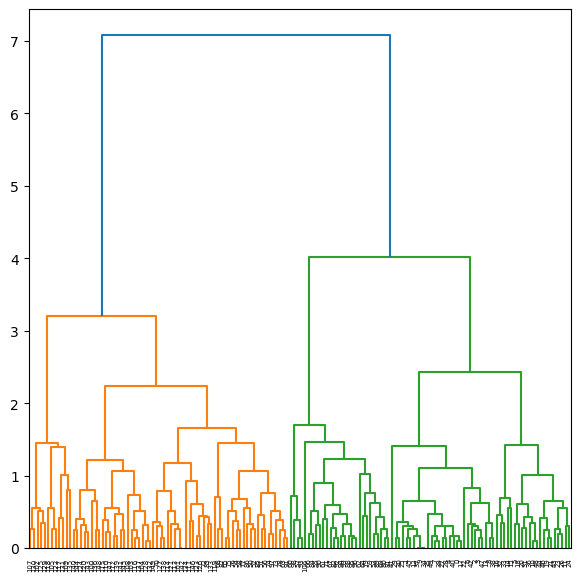
\includegraphics[width=\textwidth]{Documentos Extra/Imagenes/complete_linkage.png}
    \caption{Enlace Completo}
    \label{fig:complete_linkage}
  \end{minipage}
  \hfill
  \begin{minipage}{0.45\textwidth}
    \centering
    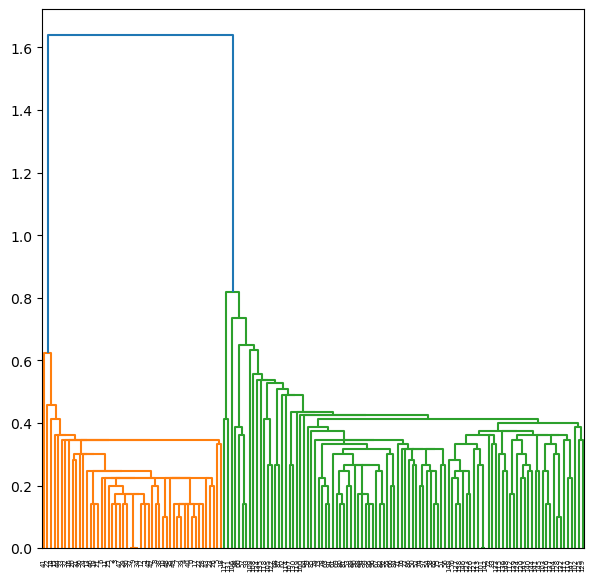
\includegraphics[width=\textwidth]{Documentos Extra/Imagenes/single_linkage.png}
    \caption{Enlace simple}
    \label{fig:single_linkage}
  \end{minipage}
 \end{figure}

\noindent Como se puede observar, el enlace completo tiende a hacer grupos más equilibrados, tendiendo a hacer una división más balanceada del espacio, mientras que el enlace simple no. Esto se traduce en que el enlazamiento completo produce grupos más esféricos mientras que el enlazamiento simple tienden a ser alargados \cite{Peña 2002}. 

\subsection{Algoritmos Particionales}

\noindent El clustering particional busca hacer una única partición que dividida las observaciones en grupos homogéneos sin definir una medida de similitud, de esta manera 

\begin{defi}
Se llama \emph{centroide} de un cluster, $C_k,\quad k=1\ldots K$ al elemento que resulta de hacer la media de todos los elementos del cluster $C_k$:
\begin{equation}
\overline{x}_{jk}=\dfrac{1}{|C_k|}\sum_{i\in C_k} x_{ij}
\end{equation}
\end{defi}

\begin{defi}
Se llama variabilidad o variación intra-cluster del cluster $C_k\quad k=1\ldots K$ a la siguiente expresión:
\begin{equation}
\mathbf{W}(C_k)=\sum_{i\in C_k}\sum_{j=1}^{p} (x_{ij}-\overline{x}_{jk})^2
\end{equation}
\noindent Esta medida también se podría dar como la media de las diferencias cuadradas entre las observaciones del cluster, pero se seleccionará esta expresión. 
\end{defi}

\noindent Una vez dadas estas definiciones y criterios se puede construir un algoritmo iterativo como es el método de K-means que se puede resumir de la siguiente manera, sabiendo el número inicial de clusters, $K$:
\begin{enumerate}
\item Se inicializa la asignación de manera aleatoria, agrupando en los $K$ clusters observaciones aleatoriamente. 
\item Se itera lo siguiente hasta que no haya cambio en los clusters:
\begin{enumerate}
\item Se calculan los centroides de cada uno de los $K$ clusters
\item Se reasignan las observaciones de acuerdo a qué centroide es más cercano según la distancia euclidiana. 
\end{enumerate}
\end{enumerate}

\begin{propo}
El algoritmo de $K$-means sólo puede mejorar el criterio de la variación dentro de clusters.\cite{Scitovski 2021}. 
\end{propo}

\noindent Estos métodos parten de una partición inicial de los datos, es decir, crean una asignación podríamos hablar de una variable discreta $y$ de tal manera que $y_i=k\Leftrightarrow \mathbf{x}_i\in C_k, i=1,\ldots, N$. Por tanto, se pueden definir las matrices $\mathbf{T},\mathbf{B},\mathbf{W}$ de manera análoga a como se construían cuando se detallaban para clasificación y también se obtenía la siguiente descomposición:
\begin{equation}
\mathbf{T}=\mathbf{B}+\mathbf{W}
\end{equation}

\noindent A estos métodos \emph{Everitt, B.S} \cite{Everitt 2011} los llama métodos de optimización, ya que buscan minimizar o maximizar distintas medidas, en el caso del algoritmo de $K$-medias se busca la minimización de la medida $tr(\mathbf{W})$.

\noindent En el caso del algoritmo de $K$-medias, se puede ver que este es un proceso que puede conducir a una minimización que no sea global de manera que tengamos que repetir de manera repetida el proceso con distintas inicializaciones para obtener el mejor resultado, en particular, \emph{Peña, D.}\cite{Peña 2002} destaca un contraste de hipótesis para elegir el número de clusters a conseguir. Todo ello basándose en los resultados de \emph{Hartigan J.A.} \cite{Hartigan 1975} el cual desarrolla en la sección 4.8 las propiedades aleatorias de cada una de las medidas seleccionadas. 



%
%\noindent Otro de los problemas de este tipo de algoritmos es que se deben conocer a priori el número de clusters en los que se quieren dividir las observaciones. Para ello \emph{Peña D.}\cite{Peña 2002} propone un contraste de hipótesis  utilizando la inercia haciéndola depender del número de clusters
%\begin{equation}
%F=\dfrac{inercia(K)-inercia(K+1)}{\frac{inercia(K+1)}{n-K-1}}
%\end{equation}
%Este cociente compara la disminución de la variación entre una partición con $K$ y $K+1$ clústers, de esta manera, puede compararse con una F con $p,p(n-K-1)$ grados de libertad, pero que en la práctica no se puede asumir las hipótesis, por tanto,  si se da un valor mayor que 10 se asume que es conveniente añadir un clúster más. 
%
%\noindent En cambio, \emph{Johnson R.A. y Wichern D.W.}\cite{Johnson 2007} proponen otra forma de contrastar la separación que no es más que 
%\begin{equation}
%F=\dfrac{}{inercia} 
%\end{equation}

